\section{Discussion}
TODO: really need a better structure
TODO: maybe put all except Spatiality and Networks, advantages and disadvantages into other paper?

\subsection{Spatiality and Networks}
When emulating the dynamics of the SIR model using an agent-based approach the question arises what we ultimately gain from doing so when we could have generated the dynamics much quicker and smoother using the SD approach. The difference is that the agent-based approach is a stochastic one and can thus also generate "degenerated" dynamics e.g. in which the disease dies out after a few steps or even can't spread from patient zero - in this case ABS is clearly a benefit as it allows to investigate \textit{alternative futures}, something not possible with SD in which the disease will never die out prematurely when there are non-zero infected agents. \\
Another advantage of ABS over the system-dynamics approach is that agents can be heterogeneous and make use of spatial- and/or network-information defining the neighbourhood. We can thus simulate the spread of the disease throughout a population which is laid out on a 2D grid or one can investigate spreading of the disease throughout a network of agents where some are vaccinated and others not. We provide already suitable environments to simulate these cases and show an example of spreading the disease on a 2D grid in Figure \ref{fig:sir_spatial}.  

\begin{figure*}
\begin{center}
	\begin{tabular}{c c}
		\begin{subfigure}[b]{0.4\textwidth}
			\centering
			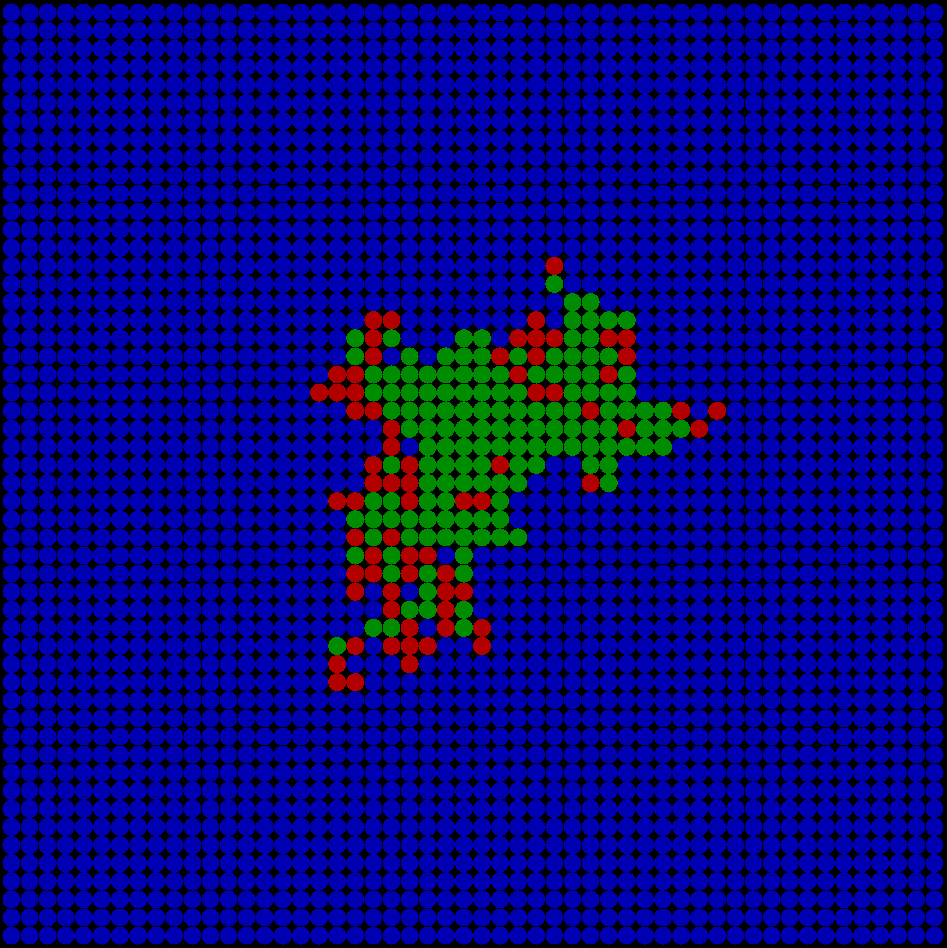
\includegraphics[width=.6\textwidth, angle=0]{./../shared/fig/spatial/SIR_spatial_52x52_92time.png}
			\caption{$t = 92$}
			\label{fig:sir_spatial_92}
		\end{subfigure}

		& 

		\begin{subfigure}[b]{0.4\textwidth}
			\centering
			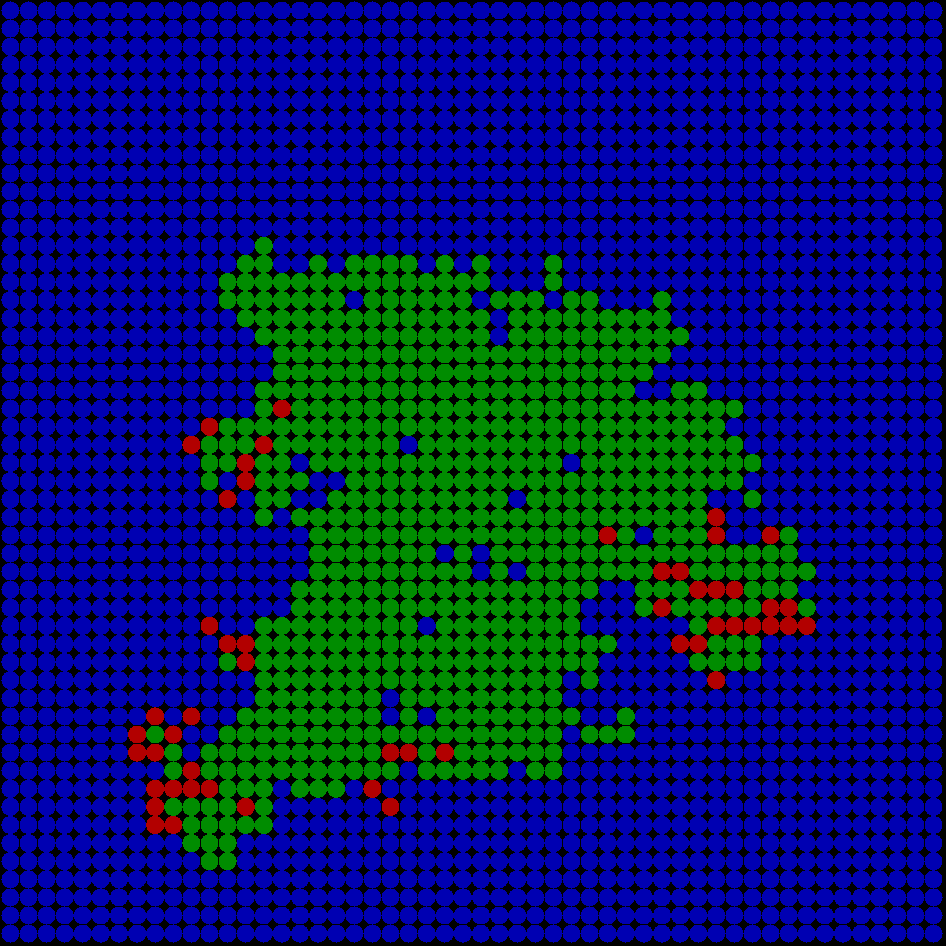
\includegraphics[width=.6\textwidth, angle=0]{./../shared/fig/spatial/SIR_spatial_52x52_200time.png}
			\caption{$t = 200$}
			\label{fig:sir_spatial_200}
		\end{subfigure}

		\\
		
		\begin{subfigure}[b]{0.4\textwidth}
			\centering
			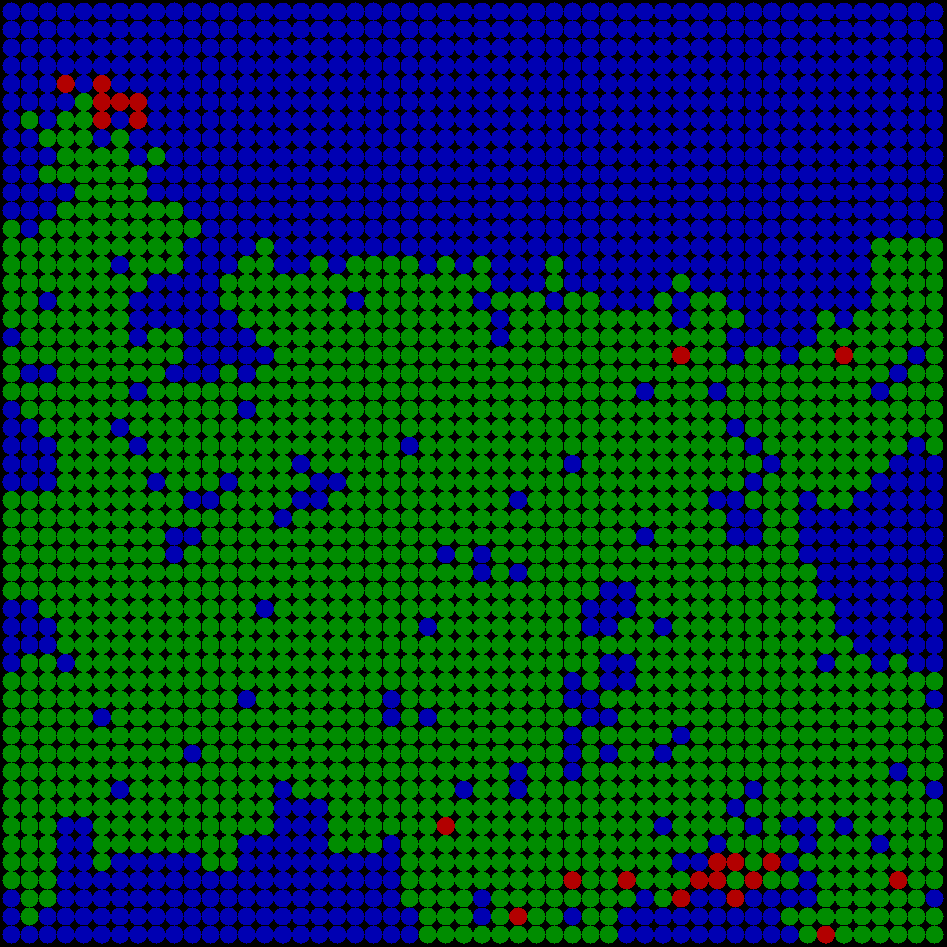
\includegraphics[width=.6\textwidth, angle=0]{./../shared/fig/spatial/SIR_spatial_52x52_440time.png}
			\caption{$t = 440$}
			\label{fig:sir_spatial_440}
		\end{subfigure}
		
		& 
		
		\begin{subfigure}[b]{0.4\textwidth}
			\centering
			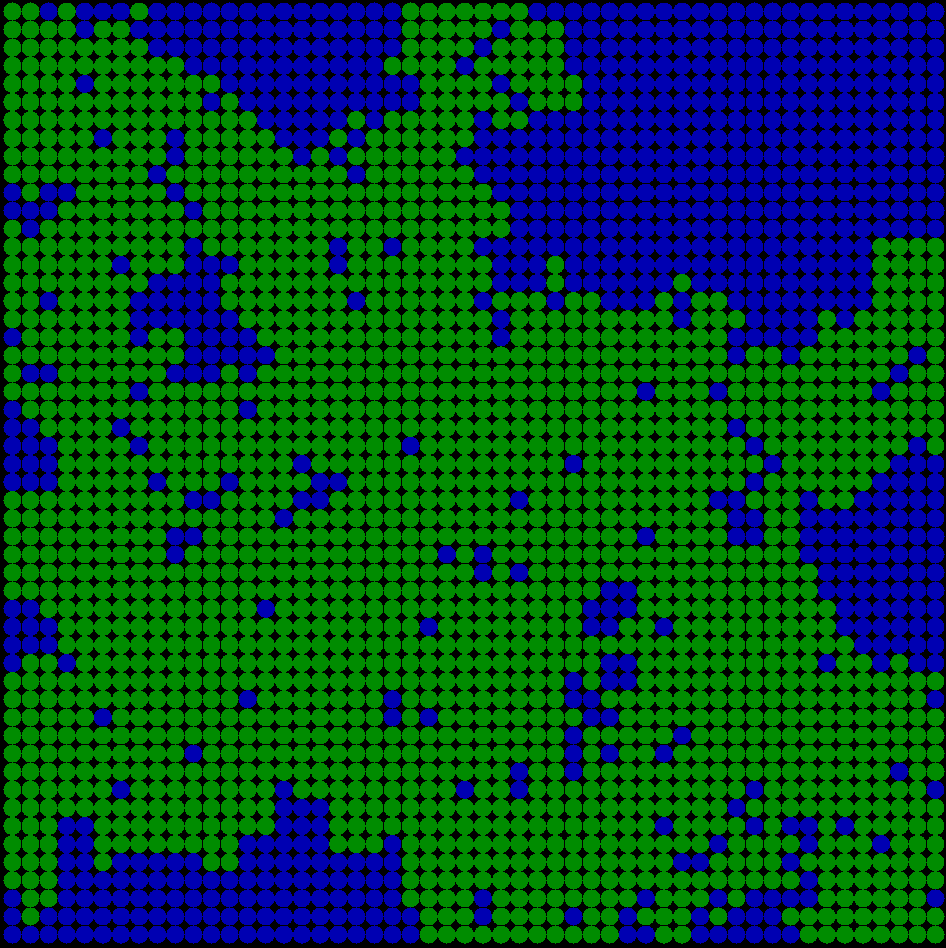
\includegraphics[width=.6\textwidth, angle=0]{./../shared/fig/spatial/SIR_spatial_52x52_873time.png}
			\caption{$t = 873$}
			\label{fig:sir_spatial_873}
		\end{subfigure}
	\end{tabular}
	
	\caption{Simulating SIR on a 52x52 grid with Moore neighbourhood using $\Delta t = 1$. Blue are susceptible, red are infected, green are recovered. The green areas act as protection as infected cannot cross the recovered border: this is particularly visible in the lower right corner of \ref{fig:sir_spatial_440} where the disease has been contained in the blue island and has no means to escape. It may seem that the few remaining infected agents in the top left corner of \ref{fig:sir_spatial_440} will die out soon but still it needs more than the already running simulation-time until the disease actually dies out with the last patient recovering at center top of \ref{fig:sir_spatial_873} at $t = 873$. The dynamics of this simulation run can be seen in Figure \ref{fig:sir_spatial_dynamics}.} 
	\label{fig:sir_spatial}
\end{center}
\end{figure*}

\begin{figure}
	\centering
	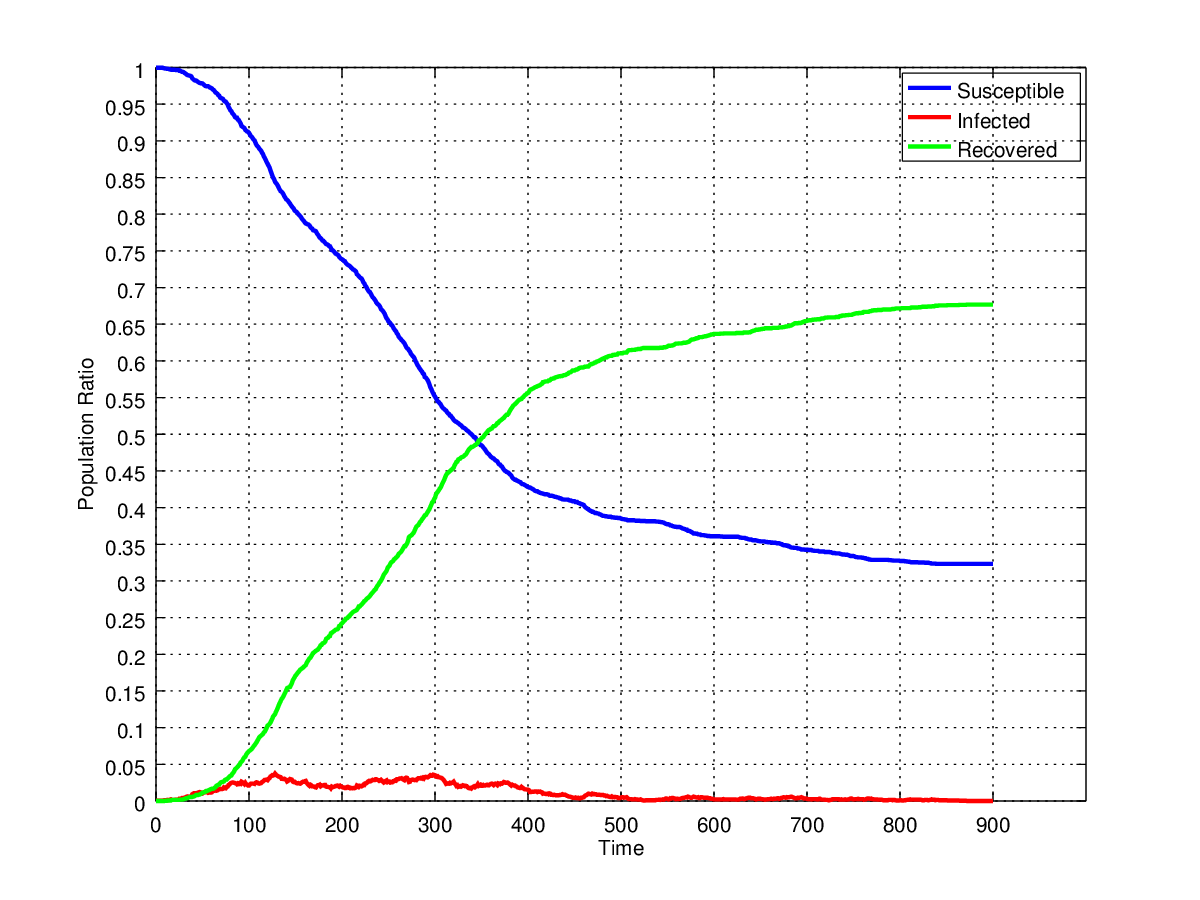
\includegraphics[width=.6\textwidth, angle=0]{./../shared/fig/spatial/SIR_spatial_dynamics_52x52_900time_1dt_parallel.png}
	\caption{Dynamics of the spatial SIR simulation from Figure \ref{fig:sir_spatial}.}
	\label{fig:sir_spatial_dynamics}
\end{figure}

Note that the dynamics of the spatial SIR simulation which are seen in Figure \ref{fig:sir_spatial_dynamics} look very different from the SD dynamics of Figure \ref{fig:sir_sd_dynamics}. This is due to a much more restricted neighbourhood which results in far fewer infected agents at a time and a lower number of recovered agents at the end of the epidemic, meaning that fewer agents got infected overall.

When using a 2D grid or network one needs to set them up in the initialization code so there is a little more work to do there but the implementation of the agents differ just in one single line, which is where the neighbourhood is picked (see line 100 of Appendix \ref{app:abs_code}). Instead of \textit{randomAgentIdMsgSource} one uses either \textit{randomNeighbourNodeMsgSource} in the case of a network or \textit{randomNeighbourCellMsgSource} in case of a 2D grid.

\subsection{Agents as Signals}
Due to the underlying nature and motivation of FRP and Yampa, agents can be seen as signals which are generated and consumed by a signal-function which is the behaviour of an agent.  If an agent does not change, the output-signal should be constant amd if the agent changes e.g. by sending a message, changing its state,... the output-signal should change as well. A dead agent then should have no signal at all.
The question is if the agents of our agent-based SIR implementation are true signals: do the dynamics stay constant when we sample the system with $\Delta t = 0$? We hypothesize that our agents are true signals, thus they should not change when time does not change because they are completely time-dependent and rely completely on time-semantics. When actually running the simulation with $\Delta t = 0$ one gets the results as seen in Figure \ref{fig:sir_abs_zero_dt}.

\begin{figure*}
\begin{center}
	\begin{tabular}{c c}
		\begin{subfigure}[b]{0.5\textwidth}
			\centering
			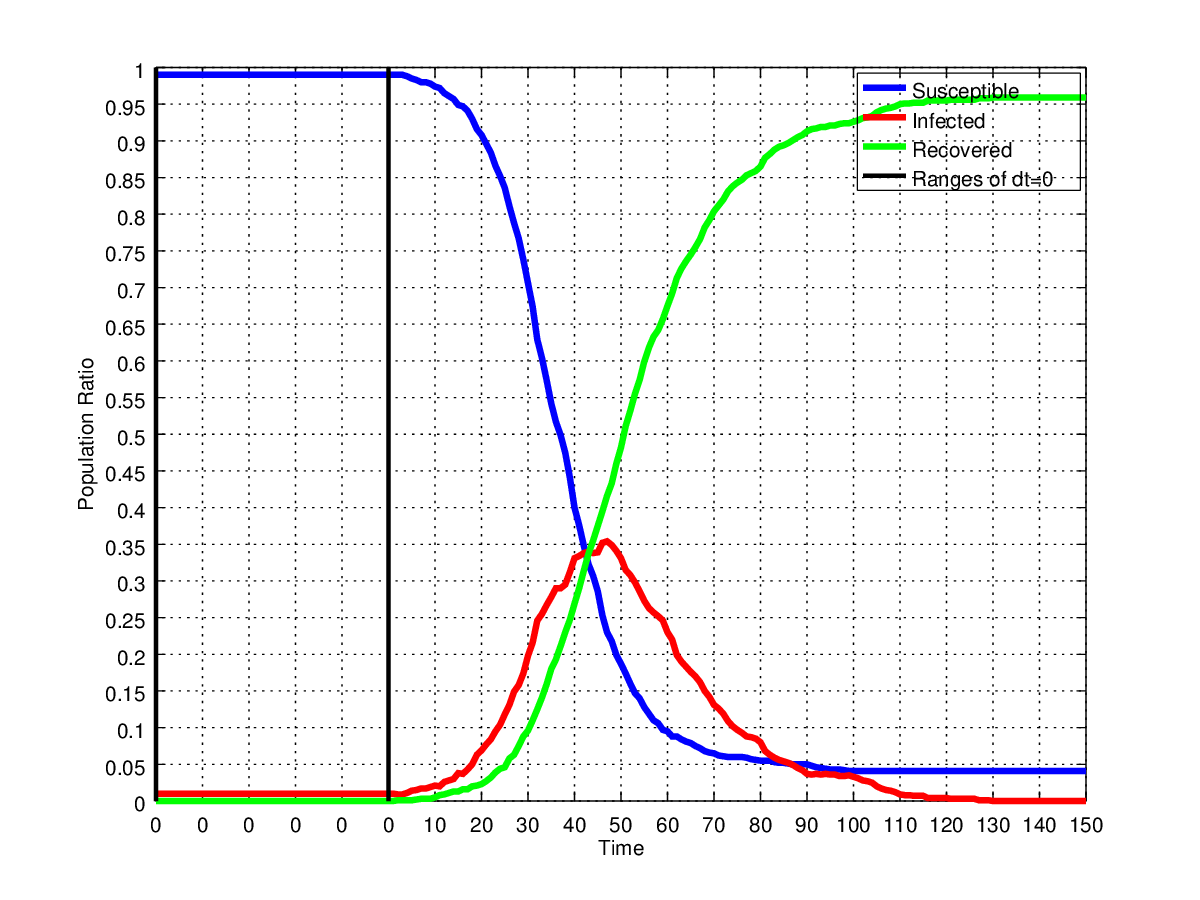
\includegraphics[width=.8\textwidth, angle=0]{./../shared/fig/dtzero/SIR_ABS_zeroDt_start.png}
			\caption{$\Delta t = 0$ from step 0 to 50.}
			\label{fig:sd_plot_10dt}
		\end{subfigure}
	
		& 
		
		\begin{subfigure}[b]{0.5\textwidth}
			\centering
			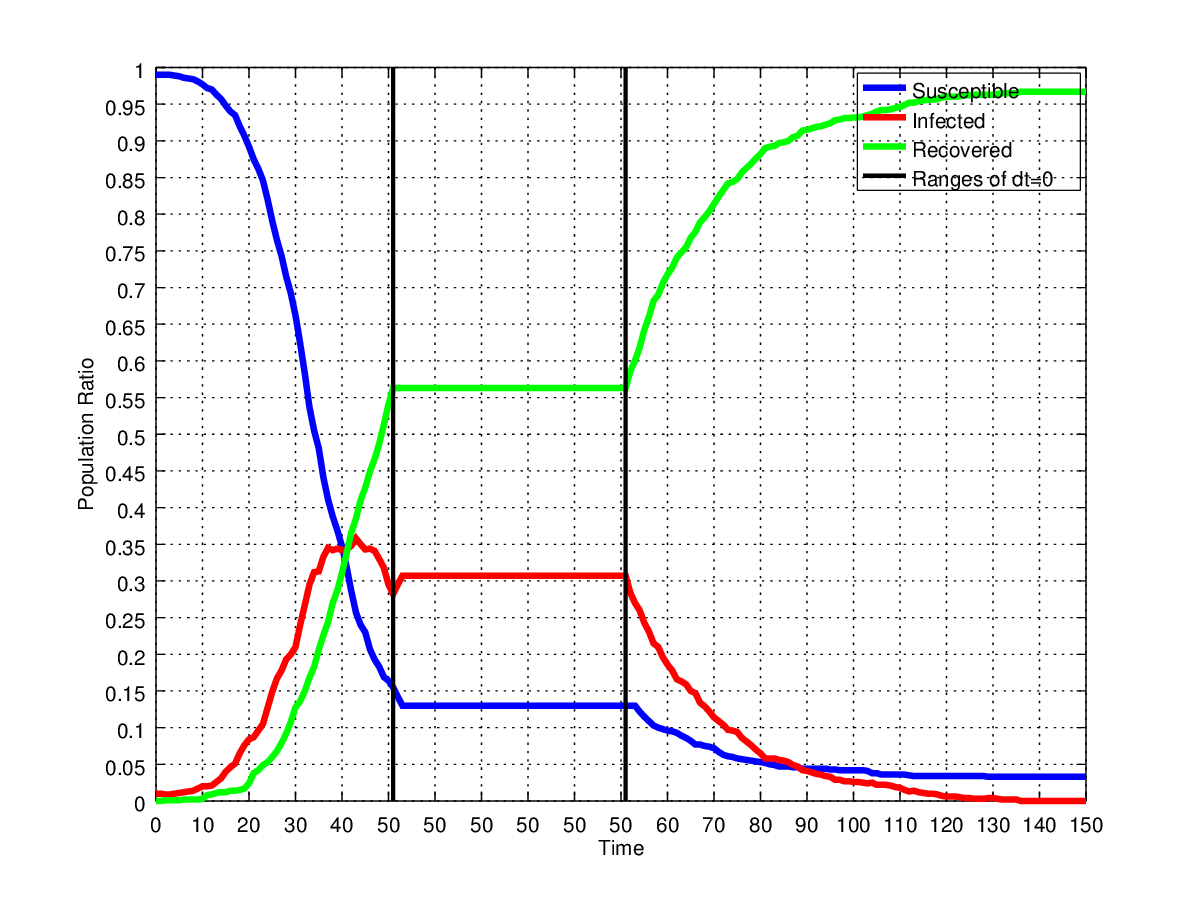
\includegraphics[width=.8\textwidth, angle=0]{./../shared/fig/dtzero/SIR_ABS_zeroDt_mid.png}
			\caption{$\Delta t = 0$ from step 51 to 101.}
			\label{fig:sd_plot_0.01dt}
		\end{subfigure}
	\end{tabular}
	
	\caption{Dynamics of agent-based SIR implementation of 1,000 agents running with $\Delta t = 1$ with ranges of $\Delta t = 0$ marked with two vertical black lines.}
	\label{fig:sir_abs_zero_dt}
\end{center}
\end{figure*}

As can be seen  the dynamics are becoming constant \textit{but} with a minor delay: infected increases a bit while susceptible decreases as can be seen in Figure \ref{fig:sir_abs_zero_dt_zoom}. This is due to the delay of message delivery which takes one $\Delta t$, independent of its value - messages are also delivered when $\Delta t = 0$. Only message-generating functions, which depend on non-zero $\Delta t$ to generate messages, will then stop generating messages. Reactive functions which act on incoming messages can still create change as they do not rely on time-semantics but just on the discrete event of a message arrival - which is the case in the transition from susceptible to infected.

\begin{figure}
	\centering
	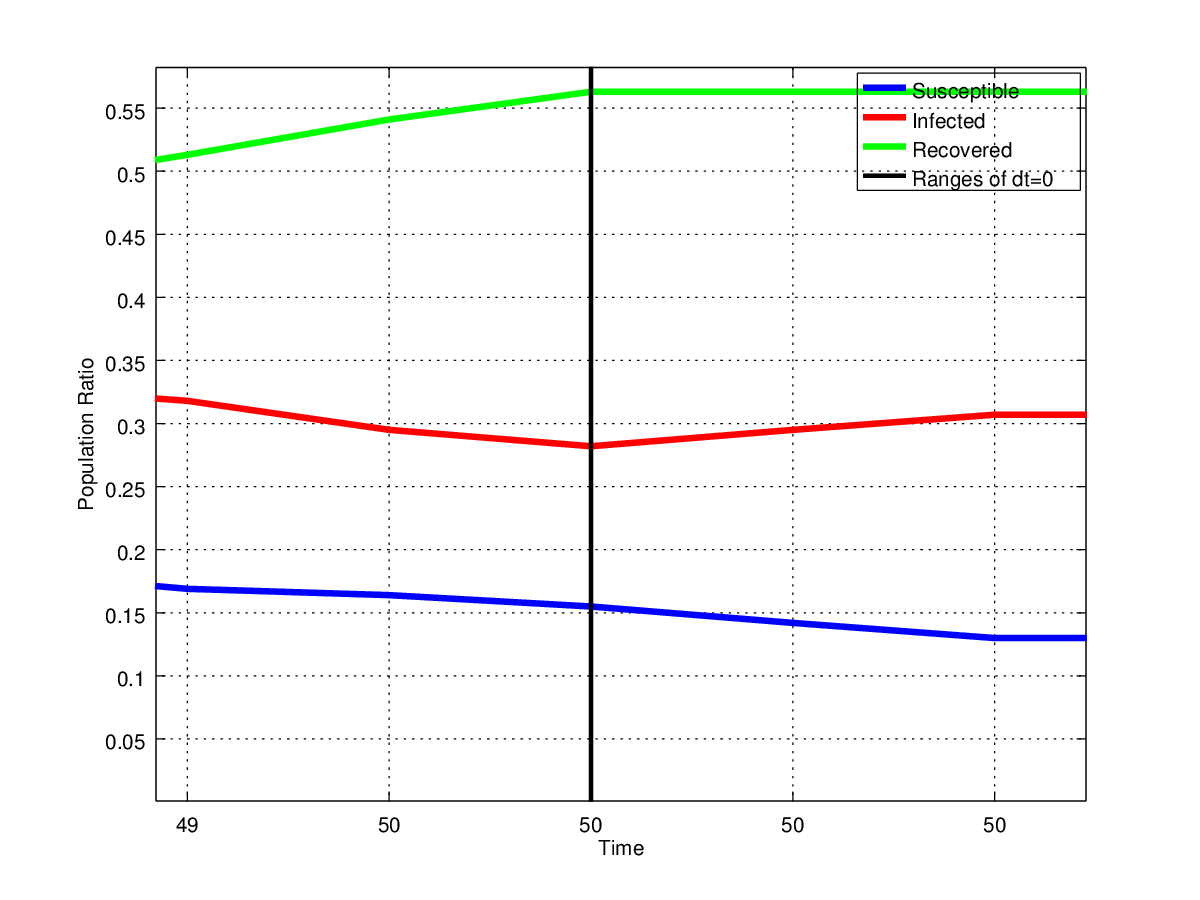
\includegraphics[width=.4\textwidth, angle=0]{./../shared/fig/dtzero/SIR_ABS_zeroDt_mid_zoom.png}
	\caption{Zoom-in to step 51, marked with the black line from where on $\Delta t = 0$ for the next 50 steps. The recovered ratio stays constant but a few agents get infected even \textit{after} having switched to $\Delta t = 0$ which happens due to the message delivery lag. After all messages have been delivered, the signal stays constant until non-zero $\Delta t$ are turned on again.}
	\label{fig:sir_abs_zero_dt_zoom}
\end{figure}

Note that agents of models with no time-semantics won't exhibit this behaviour - the dynamics will change even in case of $\Delta t = 0$ as agents act on every update and don't care about $\Delta t$ and just assume that every update occurs after $\Delta t$ independent of the actual value of it. We implemented the function \textit{doRepeatedlyEvery} which allows to transform a time-agnostic agent-behaviour into one. It is built on Yampas \textit{repeatedly} function and has the following signature:

\begin{minted}[fontsize=\footnotesize]{haskell}
doRepeatedlyEvery :: Time -> AgentBehaviour -> AgentBehaviour
\end{minted}

This function takes a time interval and an agent behaviour signal-function and returns a new agent behaviour signal-function which runs the argument signal-function every time-interval. Note that this function is subject to sampling issues too e.g. when the time-interval is very small one needs to run the simulation with a $\Delta t \leq Time$ otherwise the dynamics would show delayed activation of the agent behaviour.

\subsection{Randomness}
It is important to note that if we disable super-sampling and run the simulation for a given time \textit{t} but with two different $\Delta t$ we would end up with two different results, even if the $\Delta t$ are small enough to sample the time-dependent functions sufficiently. Also if we use super-sampling with $\Delta t = 1.0$ and create the exact same number of samples as when using no super-sampling but smaller $\Delta t$, then we also end up with different results.
The reason for this behaviour is that most of the time-dependent functions ultimately build upon drawing from random-distributions. With different $\Delta t$ we are generating a different number of random-samples, which would result in different random-number sequences which in turn ultimately leads to slightly different dynamics. When generating a plot of the dynamics this is not as visible, also this is the reason why one generates multiple replications, but this behaviour becomes strikingly apparent when simulating the SIR model on a 2D grid as can be seen in Figure \ref{fig:sir_abs_timeDeltas_randomness}.

\begin{figure*}
\begin{center}
	\begin{tabular}{c c}
		\begin{subfigure}[b]{0.4\textwidth}
			\centering
			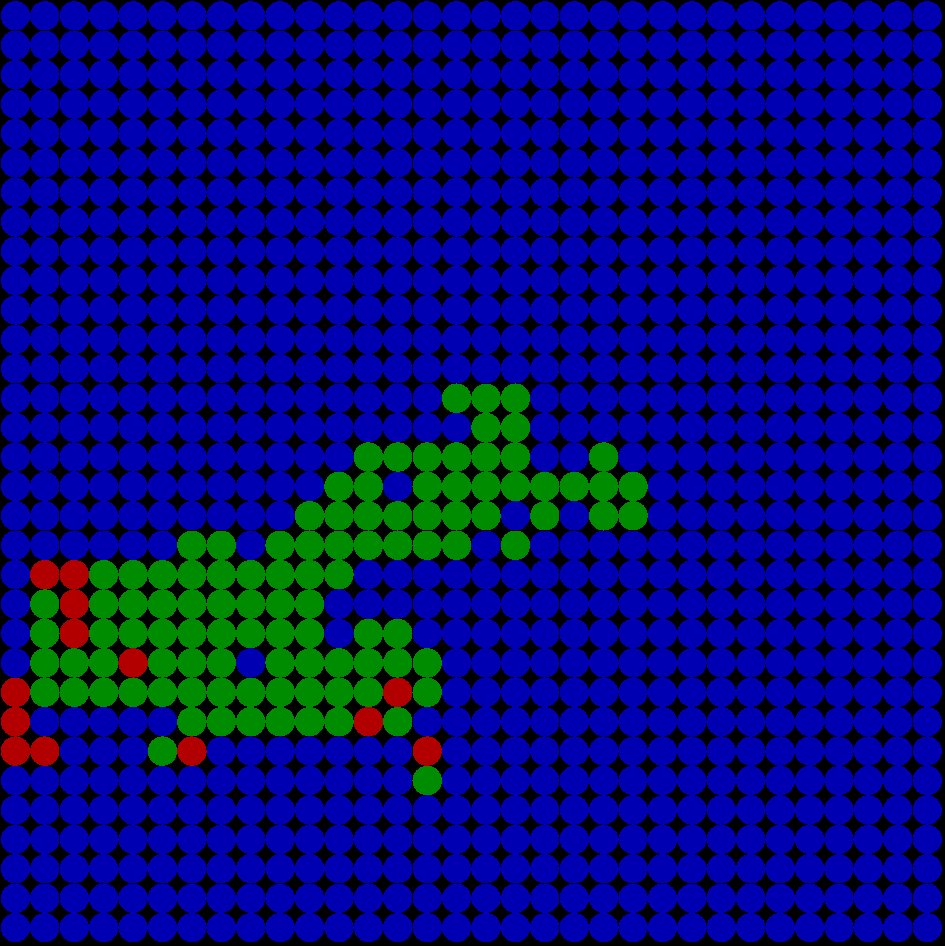
\includegraphics[width=.7\textwidth, angle=0]{./../shared/fig/randomness/SIR_32x32_200time_01delta_noSS.png}
			\caption{$\Delta t = 0.1$, no super-sampling}
			\label{fig:sir_abs_timeDeltas_randomness_dt01}
		\end{subfigure}
	
		& 
		
		\begin{subfigure}[b]{0.4\textwidth}
			\centering
			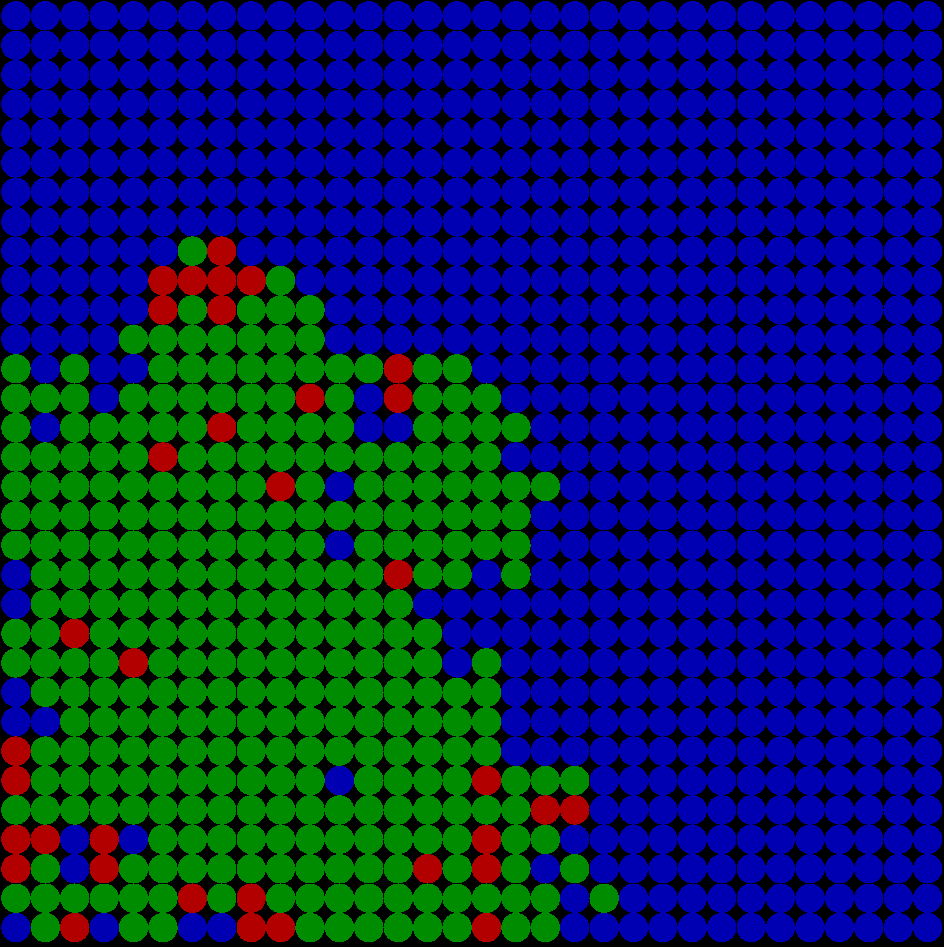
\includegraphics[width=.7\textwidth, angle=0]{./../shared/fig/randomness/SIR_32x32_200time_001delta_noSS.png}
			\caption{$\Delta t = 0.01$, no super-sampling}
			\label{fig:sir_abs_timeDeltas_randomness_dt001}
		\end{subfigure}
		
		\\

		\begin{subfigure}[b]{0.4\textwidth}
			\centering
			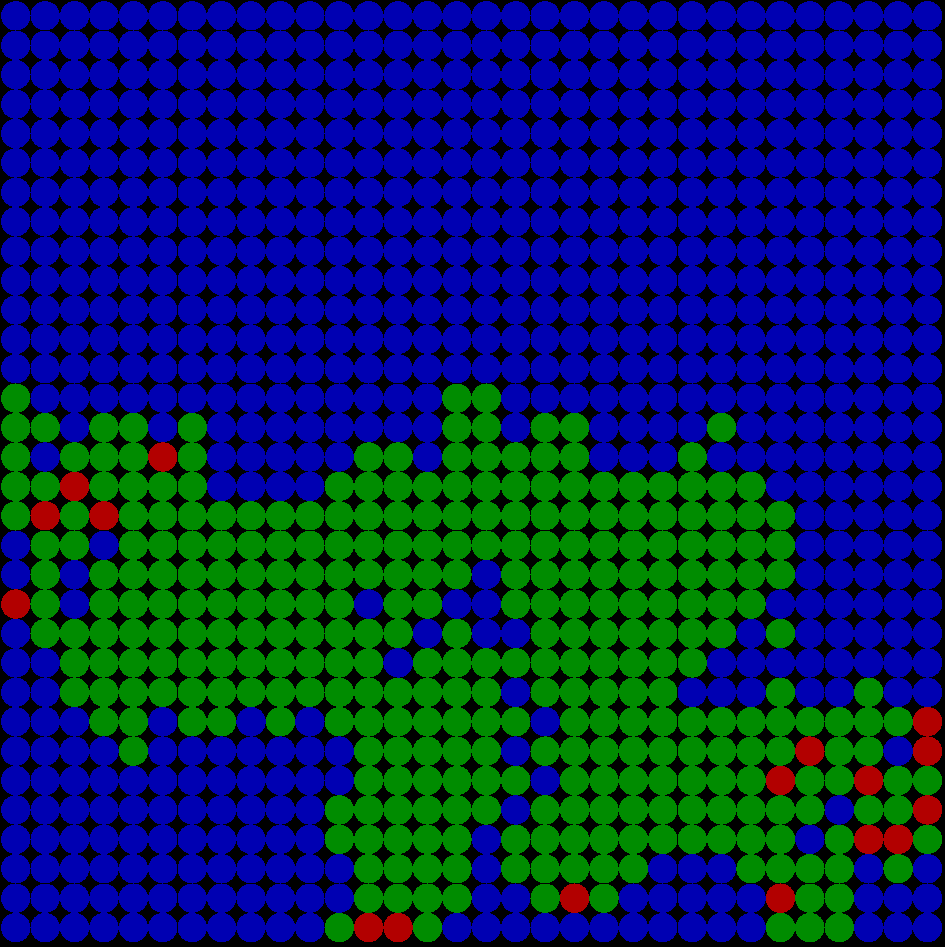
\includegraphics[width=.7\textwidth, angle=0]{./../shared/fig/randomness/SIR_32x32_200time_10delta_ss10.png}
			\caption{$\Delta t = 1.0$ with 10 super-samples}
			\label{fig:sir_abs_timeDeltas_randomness_dt10_ss10}
		\end{subfigure}
		
		&
		
		\begin{subfigure}[b]{0.4\textwidth}
			\centering
			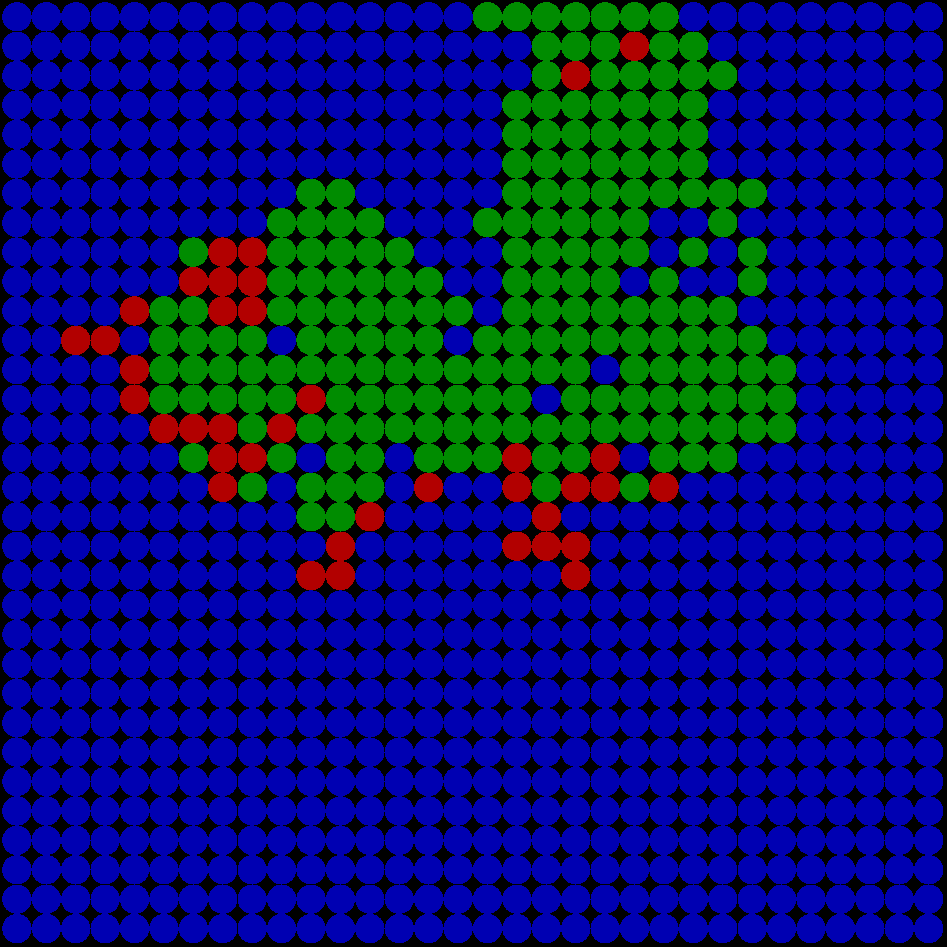
\includegraphics[width=.7\textwidth, angle=0]{./../shared/fig/randomness/SIR_32x32_200time_10delta_ss100.png}
			\caption{$\Delta t = 1.0$ with 100 super-samples}
			\label{fig:sir_abs_timeDeltas_randomness_dt10_ss100}
		\end{subfigure}
	\end{tabular}
	
	\caption{Comparing results on 32x32 grid after $t = 200$ but with different $\Delta t$ and different number of super-samples.}
	\label{fig:sir_abs_timeDeltas_randomness}
\end{center}
\end{figure*}

\subsection{Advantages}
We now look at a number of advantages this functional reactive approach to ABS has over to the traditional imperative, object-oriented implementation approaches done in Phyton, Java, C++.

\subsubsection{Continuous Time}
It seems that in our approach we combine the benefits of SD and ABS: we have continuous time-semantics but with individual, heterogenous agents.

\subsubsection{Code close to specification}
When looking at the code of the agent-based implementation in Appendix \ref{app:abs_code} and SD implementation in Appendix \ref{app:sd_code}, both look very much like a specification. By creating this EDSL which allows to express powerful time-semantics it is possible to now create an ABS in a declarative style in Haskell where the agent-implementation looks very much like a model-specification thus being correct by definition.
We claim that this is not only true for models with time-semantics but also with models which lack time-semantics and resemble a more imperative style of behaviour. We can also capture this using monadic programming using the State Monad for which we provide EDSL primitives as well which support all necessary operations in a monadic context.

\subsubsection{Being pure}
Because no part of the simulation runs in the IO monad and we do not use unsafePerformIO we can rule out a serious class of bugs caused by implicit data-dependencies and side-effects which can occur in traditional imperative implementations. Note that we actually use unsafePerformIO when one wants to generate unique agent-ids for new agents which are created during the simulation. This is necessary because in this case we need to guarantee that two invocations will result in two different ids, which would be difficult / impossible when running the simulation in the \textit{parallel} update-strategy. This is not a problem as long as an agent does not rely on the absolute value of an agent-id but just uses it as an opaque identifier for messaging.
Also we can statically guarantee the reproducibility of the simulation. Within the agents there are no side effects possible which could result in differences between same runs (e.g. file access, networking, threading, random-number seeding). Every agent has access to its own random-number generator, allowing randomness to occur in the simulation but the random-generator seed is fixed in the beginning and can never be changed within an agent to come from e.g. the current system time, which would require to run within the IO Monad. This means that after initialising the agents, which \textit{could} run in the IO Monad, the simulation itself runs completely deterministic.
We provide functionality to render the output to a window (using the Gloss library) or writing to a text-file, meaning, parts of the simulation would run in the IO Monad. Here we rely on Yampas \textit{reactimate} function which provides a well-defined way of communicating with the world in such a system. This function provides the $\Delta t$ for the next step, which \textit{could} come from IO Monad but we forbid this and keep the $\Delta t$ always fixed, thus removing another source of non-reproducibility where $\Delta t$ is influenced by sytem dependent non deterministic rendering-performance every step as happens in games or described by \cite{perez_testing_2017} in the context of FRP.

\subsubsection{Robust time handling}
The actual $\Delta t$ is never visible leads to an even more declarative style and supports the EDSL greatly. This also makes it impossible to mess around with time.

\subsubsection{Replications}
We nearly get replications for free without having to worry about side-effects and can even run them in parallel without headaches.

\subsection{Disadvantages}
We identify two main disadvantages.

\subsubsection{Performance}
Performance is currently no where near imperative object-oriented implementations. The reason for this is that we don't have in-place updates of data-structures and make no use of references. This results in lots of copying which is simply not necessary in the imperative languages with implicit effects. Also it is much more difficult to reason about time and space in our approach. Thus we see performance clearly as the main drawback of the functional approach and the only real advantage of the imperative approach over our.

\subsubsection{Steep learning curve}
Our approach is quite advanced in three ways. First it builds on the already quite involved FRP paradigm. Second it forces one to think properly of time-semantics of the model, how to sample it, how small $\Delta t$ should be and whether one needs super-sampling or not and if yes how many samples one should take. Third it requires to think about agent-interaction and update-strategies, whether one should use conversations which forces one to run sequentially or if one can run agents in parallel and use normal messaging which incurs a time-delay which in turn would need to be considered when setting the $\Delta t$.